%%%%%%%%%%%%%%%%%%%%%%%%%%%%%%%%%%%%%%%%%
% Journal Article
% LaTeX Template
% Version 1.4 (15/5/16)
%
% This template has been downloaded from:
% http://www.LaTeXTemplates.com
%
% Original author:
% Frits Wenneker (http://www.howtotex.com) with extensive modifications by
% Vel (vel@LaTeXTemplates.com)
%
% License:
% CC BY-NC-SA 3.0 (http://creativecommons.org/licenses/by-nc-sa/3.0/)
%
%%%%%%%%%%%%%%%%%%%%%%%%%%%%%%%%%%%%%%%%%

%----------------------------------------------------------------------------------------
%	PACKAGES AND OTHER DOCUMENT CONFIGURATIONS
%----------------------------------------------------------------------------------------

%\documentclass{article}
%\documentclass[oneside,twocolumn]{article}
\documentclass[oneside,onecolumn]{article}

\usepackage{blindtext} % Package to generate dummy text throughout this template 
\usepackage{multicol}
\usepackage[sc]{mathpazo} % Use the Palatino font
\usepackage[T1]{fontenc} % Use 8-bit encoding that has 256 glyphs
\linespread{1.05} % Line spacing - Palatino needs more space between lines
\usepackage{microtype} % Slightly tweak font spacing for aesthetics

%\usepackage[english]{babel} % Language hyphenation and typographical rules
\usepackage[spanish]{babel}
\usepackage[hmarginratio=1:1,top=32mm,columnsep=20pt]{geometry} % Document margins
\usepackage[hang, small,labelfont=bf,up,textfont=it,up]{caption} % Custom captions under/above floats in tables or figures
\usepackage{booktabs} % Horizontal rules in tables

\usepackage{lettrine} % The lettrine is the first enlarged letter at the beginning of the text

\usepackage{listings} % Required for insertion of code

\usepackage{enumitem} % Customized lists
\setlist[itemize]{noitemsep} % Make itemize lists more compact

\usepackage{abstract} % Allows abstract customization
\renewcommand{\abstractnamefont}{\normalfont\bfseries} % Set the "Abstract" text to bold
\renewcommand{\abstracttextfont}{\normalfont\small\itshape} % Set the abstract itself to small italic text

\usepackage{titlesec} % Allows customization of titles
\renewcommand\thesection{\Roman{section}} % Roman numerals for the sections
\renewcommand\thesubsection{\roman{subsection}} % roman numerals for subsections
\titleformat{\section}[block]{\large\scshape\centering}{\thesection.}{1em}{} % Change the look of the section titles
\titleformat{\subsection}[block]{\large}{\thesubsection.}{1em}{} % Change the look of the section titles

\usepackage{fancyhdr} % Headers and footers
\pagestyle{fancy} % All pages have headers and footers
\fancyhead{} % Blank out the default header
\fancyfoot{} % Blank out the default footer
%\fancyhead[C]{Running title $\bullet$ May 2016 $\bullet$ Vol. XXI, No. 1} % Custom header text
\fancyfoot[RO,LE]{\thepage} % Custom footer text

\usepackage{titling} % Customizing the title section

\usepackage{hyperref} % For hyperlinks in the PDF

\usepackage{listings}
\usepackage{algorithm2e}
\usepackage{graphicx}
\usepackage[dvipsnames]{xcolor}
\definecolor{codegreen}{rgb}{0,0.6,0}
\definecolor{codegray}{rgb}{0.5,0.5,0.5}
\definecolor{codepurple}{rgb}{0.58,0,0.82}
\definecolor{backcolour}{rgb}{1,1,1}
\lstdefinestyle{mystyle}{
    backgroundcolor=\color{backcolour},   
    commentstyle=\color{codegreen},
    keywordstyle=\color{magenta},
    numberstyle=\tiny\color{codegray},
    stringstyle=\color{codepurple},
    basicstyle=\ttfamily\footnotesize,
    breakatwhitespace=false,         
    breaklines=true,                 
    captionpos=b,                    
    keepspaces=true,                 
    numbers=left,                    
    numbersep=5pt,                  
    showspaces=false,                
    showstringspaces=false,
    showtabs=false,                  
    tabsize=2
}
\renewcommand{\lstlistingname}{Código}% Listing -> Algorithm
\lstset{style=mystyle}

\usepackage[utf8]{inputenc} % Required for inputting international characters
\usepackage[T1]{fontenc} % Output font encoding for international characters
\usepackage[
backend=biber,
style=alphabetic,
sorting=ynt
]{biblatex}
\addbibresource{BALLADO_LUIS_CONTROL_NOLINEAL.bib} %Import the bibliography file

\usepackage{amsmath}
%----------------------------------------------------------------------------------------
%	TITLE SECTION
%----------------------------------------------------------------------------------------

\setlength{\droptitle}{-4\baselineskip} % Move the title up

\pretitle{\begin{center}\Huge\bfseries} % Article title formatting
\posttitle{\end{center}} % Article title closing formatting
\title{Control no lineal} % Article title
\author{%
\textsc{Luis Alberto Ballado Aradias} \\%\thanks{A thank you or further information} \\[1ex] % Your name
\normalsize Cinvestav Unidad Tamaulipas \\ % Your institution
\normalsize {luis.ballado@cinvestav.mx} % Your email address
%\and % Uncomment if 2 authors are required, duplicate these 4 lines if more
%\textsc{Jane Smith}\thanks{Corresponding author} \\[1ex] % Second author's name
%\normalsize University of Utah \\ % Second author's institution
%\normalsize \href{mailto:jane@smith.com}{jane@smith.com} % Second author's email address
}
\date{\today} % Leave empty to omit a date
\renewcommand{\maketitlehookd}{%
  \begin{abstract}
    \noindent El presente trabajo describe la implementación de un control no lineal con uso de la odometría para un robot móvil de tipo diferencial y su implementación utilizando un robot LEGO NXT bajo el lenguaje NXC (Not eXactly C) para la navegación de entre un punto inicial y final. El control no lineal se refiere a la técnica de controlar sistemas con comportamiento no lineal, es decir, sistemas cuyas relaciones de entrada-salida no pueden representarse mediante una  relación lineal simple e implica el uso de técnicas avanzadas de modelado y control para lograr el control deseado del sistema. Este tipo de control se utiliza en una amplia variedad de aplicaciones, desde el control de procesos industriales hasta la robótica y la navegación autónoma.
  \end{abstract}
}

%----------------------------------------------------------------------------------------

\begin{document}

% Print the title
\maketitle

%----------------------------------------------------------------------------------------
%	ARTICLE CONTENTS
%----------------------------------------------------------------------------------------
\section{Introducción}

\lettrine[nindent=0em,lines=3]{L}a teoría de sistemas de control se ocupa del análisis y el diseño de componentes interactuantes de un sistema en una configuración que brinde un comportamiento deseado. La configuración esencial usada en teoría de sistemas de control se basa en el concepto fundamental de realimentación, que consiste en el proceso de medir las variables de interés en el sistema y usar esa información para controlar su comportamiento. La teoría y la práctica del control tienen un amplio rango de aplicaciones en los campos de la ingeniería aeronáutica, química, mecánica, ambiental, civil y eléctrica, así como en muchas otras disciplinas no ingenieriles. Las ventajas del control eficiente en la industria son inmensas, e incluyen mejoras en la calidad de los productos, reducción en el consumo de energía, minimización de los material de desecho, mayores niveles de seguridad y reducción de la contaminación.\\

El punto de partida en el análisis de un sistema de control es su representación por un modelo matemático, generalmente como un operador entre entradas y salidas del sistema, o como un conjunto de ecuaciones diferencia y/o diferenciales. La mayoría de los modelos matemáticos usados tradicionalmente por teóricos y prácticos del control son lineales. De hecho, los modelos lineales son mucho más manejables que los no lineales, y pueden representar en forma precisa el comportamiento de sistemas reales en muchos casos útiles.\\

La principal dificultad radica en el hecho de que los sistemas no lineales no pueden ser analizados mediante las técnicas tradicionales de la teoría de control lineal, que se basan en la linealidad y la invariancia del sistema. En lugar de ello, se requieren herramientas matemáticas avanzadas como la teoría de sistemas dinámicos, la teoría de control óptimo, la teoría de la retroalimentación no lineal y la teoría de estabilidad no lineal para analizar y diseñar sistemas de control no lineal.\\

El control no lineal juega un papel importante en la robótica móvil, que se ocupa del diseño y la implementación de robots que pueden moverse de manera autónoma en entornos desconocidos. En este contexto, los sistemas de control no lineal son fundamentales para garantizar que el robot pueda navegar de manera segura y eficiente en un entorno cambiante y a menudo impredecible.\\

En la robótica móvil, los sistemas de control no lineal se utilizan para controlar la velocidad, la posición y la orientación del robot, y para hacer que el robot siga una trayectoria deseada. Estos sistemas se basan en técnicas avanzadas de modelado y control, como el control por realimentación no lineal, el control adaptativo y el control por modos deslizantes.\\

\subsection{Sistema de Control} %https://www.oposinet.com/temario-de-tecnologia/temario-4-tecnologia/tema-65b-sistemas-de-control-elementos-componentes-variables/

Un sistema de control es una combinación de componentes que actúan conjuntamente por medio de una serie de variables para proporcionar una respuesta acerca del propio comportamiento del sistema.\\

El control del sistema consiste en la actuación a partir de unas variables o señales de entrada. Para la representación gráfica de un sistema se utilizan bloques en el que las variables que actúan sobre el sistema (entradas) se indican con flechas que entran hacia el bloque, mientras que las variables producidas por el sistema (salidas) se indican mediante flechas que salen del bloque. Los tipos de sistema de control pueden ser, según se realice la acción de control.\\

\begin{enumerate}
\item \textbf{Sistema de control en lazo abierto} en estos sistemas, la única variable que se tiene en cuenta en la acción de control, es la señal de entrada. La señal de salida, no actúa de ninguna manera sobre el sistema. En consecuencia, no existe ninguna relación entre la respuesta del sistema y las variables de entrada.
\item \textbf{Sistema de control en lazo cerrado} en estos sistemas, tanto la entrada de referencia como muestras de la señal de salida, actúan sobre la acción de control, es decir, se realiza una realimentación de la señal en la salida a la entrada del sistema. Esta retroalimentación tiene como finalidad, ir controlando la salida y minimizar el error que puede producirse frente a perturbaciones que afecten al sistema, obteniendo con más seguridad la señal deseada a la salida.
\end{enumerate}

\subsection{Ley de Control}

La teoría de estabilidad juega un rol central en teoría de sistemas e ingeniería. En sistemas dinámicos existen distintos tipos de problemas de estabilidad. La estabilidad de puntos de equilibrio generalmente se caracteriza en el sentido de Lyapunov. \\

Un punto de equilibrio se dice estable si todas las soluciones que se inicien en las cercanías del punto de equilibrio permanecen en las cercanías del punto de equilibrio; de otro modo el punto de equilibrio es inestable. Un punto de equilibrio se dice asintóticamente estable si todas las soluciones que se inicien en las cercanías del punto de equilibrio no sólo permanecen en las cercanías del punto de equilibrio, sino que además tiendan hacia el equilibrio a medida que el tiempo se aproxima a infinito.

%------------------------------------------------

\section{Ley de Control aplicado en el Robot LEGO}

Sea la \textbf{planta} el ROBOT a controlar, donde $xf, yf, \Theta_{f}$ son la entrada de control y $x, y. \Theta$ las posiciones finales a las que queremos llegar.

\begin{figure}[h]
  \centering
  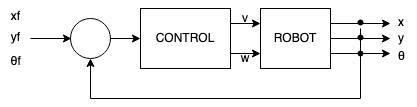
\includegraphics[scale=0.7]{graficos/bloque.png}
  \caption{Diagrama Control Lazo Cerrado}
\end{figure}

\[\dot{x} = v cos \Theta \qquad \dot{y} = v sin \Theta \dot{\Theta} = \omega \]

Un vector de error compuesto por una distancia \textbf{a} y un ángulo \textbf{$\alpha$} 

\begin{figure}[h]
  \centering
  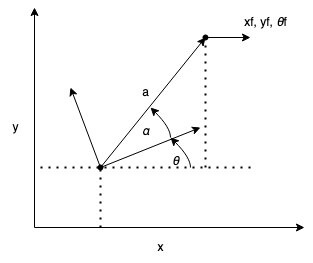
\includegraphics[scale=0.7]{graficos/grafico.png}
  \caption{Sistema}
\end{figure}

podemos ver $\Theta_{error}$ como: \\
\[ \Theta_{error} = \Theta + \alpha = tg \frac{ye}{xe} \]

consideramos nuestro vector de error:

\[ a = \sqrt{(xf-x)^{2}+(yf-y)^2} = \sqrt{x_{error}^{2} + y_{error}^2} \]

\[ \alpha = tg^{-1} \frac{y_{error}}{x_{error}} - \Theta\]

\textbf{Dinámica del error} $\dot{a}$, $\dot{\alpha}$ en función de v, w

\[ a = (x_{e}^{2} + y_{e}^{2})^{\frac{1}{2}}\]

\[ \dot{a} = \frac{\partial a}{\partial x_{error}}*\dot{x_{error}} + \frac{\partial a}{\partial y_{error}}*\dot{y_{error}}\]

\[ = \frac{1}{2} (x_{error}^{2} + y_{error}^{2})^{-\frac{1}{2}}*(2x_{error})*\dot{x_{error}} + \frac{1}{2} (x_{error}^{2}+y_{error}^2)^{-\frac{1}{2}}(2y_{error})*\dot{y_{error}}\]

\section{Resultados}

Random citation \cite{einstein:1} embeddeed in text.
%------------------------------------------------
\section{Conclusiones}


%----------------------------------------------------------------------------------------
%	REFERENCE LIST
%----------------------------------------------------------------------------------------

\begin{thebibliography}{0} % Bibliography - this is intentionally simple in this template

  \bibliography{BALLADO_LUIS_CONTROL_NOLINEAL} 
      
\end{thebibliography}

%----------------------------------------------------------------------------------------

\end{document}
